%% LaTeX template for BSc Computing for Games final year project dissertations
%% by Edward Powley
%% Games Academy, Falmouth University, UK

%% Based on:
%% bare_jrnl.tex
%% V1.4b
%% 2015/08/26
%% by Michael Shell
%% see http://www.michaelshell.org/
%% for current contact information.
%%
%% This is a skeleton file demonstrating the use of IEEEtran.cls
%% (requires IEEEtran.cls version 1.8b or later) with an IEEE
%% journal paper.
%%
%% Support sites:
%% http://www.michaelshell.org/tex/ieeetran/
%% http://www.ctan.org/pkg/ieeetran
%% and
%% http://www.ieee.org/

%%*************************************************************************
%% Legal Notice:
%% This code is offered as-is without any warranty either expressed or
%% implied; without even the implied warranty of MERCHANTABILITY or
%% FITNESS FOR A PARTICULAR PURPOSE! 
%% User assumes all risk.
%% In no event shall the IEEE or any contributor to this code be liable for
%% any damages or losses, including, but not limited to, incidental,
%% consequential, or any other damages, resulting from the use or misuse
%% of any information contained here.
%%
%% All comments are the opinions of their respective authors and are not
%% necessarily endorsed by the IEEE.
%%
%% This work is distributed under the LaTeX Project Public License (LPPL)
%% ( http://www.latex-project.org/ ) version 1.3, and may be freely used,
%% distributed and modified. A copy of the LPPL, version 1.3, is included
%% in the base LaTeX documentation of all distributions of LaTeX released
%% 2003/12/01 or later.
%% Retain all contribution notices and credits.
%% ** Modified files should be clearly indicated as such, including  **
%% ** renaming them and changing author support contact information. **
%%*************************************************************************


\documentclass[journal]{IEEEtran}

\usepackage{graphicx}
% Insert additional usepackage commands here
\usepackage[hyphens]{url} % <===========================================
\usepackage[hidelinks]{hyperref} % Allows clickable reference lists
\usepackage[none]{hyphenat} %Stops breaking up words in table
\usepackage{cite}
\usepackage{listings}
\usepackage[table,pdftex,dvipsnames]{xcolor} 

\begin{document}
%
% paper title
% Titles are generally capitalized except for words such as a, an, and, as,
% at, but, by, for, in, nor, of, on, or, the, to and up, which are usually
% not capitalized unless they are the first or last word of the title.
% Linebreaks \\ can be used within to get better formatting as desired.
% Do not put math or special symbols in the title.
\title{ How Will a Mixed-Initiative Level Designer that Predict User Requirements Affect the Size and Speed of the Levels Created?}
%
%
% author name

\author{Tristan Barlow-Griffin}

% The paper headers -- please do not change these, but uncomment one of them as appropriate
% Uncomment this one for COMP320
\markboth{COMP320: Research Review and Proposal}{COMP320: Research Review and Proposal}
% Uncomment this one for COMP360
% \markboth{COMP360: Dissertation}{COMP360: Dissertation}

% make the title area
\maketitle

% As a general rule, do not put math, special symbols or citations
% in the abstract or keywords.
\begin{abstract}
This paper builds upon a feature request by users in Alvarez~\textit{et al}\cite{alvarez2018fostering} study into a mixed-initiative level design tool. 
\end{abstract}




\markboth{COMP320: Research Review and Proposal}{COMP320: Research Review and Proposal}

\section{Introduction} \label{intro}
\IEEEPARstart{T}{his} research project will look whether a prototyping tool that predict user requirements will increase the size and speed of levels designed. A prototype is the initial design of an object \cite{prototype}. The prototyping phase of a project is used to quickly test certain aspect of a products' design so the designer can identify and clear up any problems\cite{budde1992prototyping}.Fullerton \textit{et all} \cite[p.~150]{fullerton2004game} state there are two kinds of prototyping in games: Physical and Software prototypes. Since this book was published back in 2004, the accessibility of software tools to help prototyping has increased. The author of \cite[p.~164]{fullerton2004game} also describes level editors as a good way to prototype levels. \textit{Unreal Engine 4} (UE4) implement their own version of a level editor. Within this editor the designers can create basic geometry scaling them to fit their needs as well as addition custom meshes and programmable objects.

This paper looks to build upon  a normal level editor by adding a Mixed-Initiative component that will predict the users requirements. The component will aim to reduce the time it takes to produce a level prototype. As discussed above the prototyping phase is meant to test a design, the less time and resources required to produce an artefact that can demonstrate the proposed design the better. Beyond the benefit of saving time, the less time a designer puts into a particular design the less attached to the design they become. When collaborating in a group, differing opinions can cause different constraints to be set on the design of a level. While a given design may satisfy the original designers set constraints, the prototype may have to be discarded as it did not meet the other requirements set by the team. Identifying and discarding concepts early in development can save a lot of time and energy \cite[p.489]{stempfle1999thinking} and arguable may reduce the negative impacts to interpersonal relations that idea dismissal may have. 

\section{Related Work}
The main focus of this literature review will be on prediction methods. For the research into prediction methods the scope went beyond just game design as their were limited cases of prediction methods to be found. To discover whether mixed-initiative tools really have a place in level design the selection of the prediction method must be optimal. When researching prediction methods scoping considerations have been taken into account. Some prediction methods have been the centre of studies with far more resources than this project. Prediction methods referenced are not cutting edge in the field.  The definition of mixed-initiative used in this paper will also be defined in  Section~\ref{MI}.  Also in Section~\ref{MI} mixed-Initiative tools are group into two broad categories using Liapis~\textit{et al}\cite{liapis2016mixed} definition. By defining these groups it is easier to distinguish between the most common type of mixed-initiative tool and the type of tool this paper focuses on.  n Section~\ref{UI} is an evaluation of the current state of mixed-initiative level designers being used. Using their feedback to identify features that if implemented could help to speed up the rapid prototyping phase. 

\subsection{Mixed-initiative} \label{MI}
The term mixed-initiative was first introduced by Jaime R \cite{carbonell1970mixed}.
It describes a process where by a computer and a human designer work together to achieve a goal. Other definitions of mixed-initiative build on the idea of human computer co-creativity. This paper will use the first definition of mixed-initiative presented. As it is easier to define and the definition of creativity is a very complex matter in itself. 

There are two broad categories that MI tools can be grouped into, Interactive evolution and Computer-aided design \cite{liapis2016mixed}. 
\begin{itemize}
    \item \textit{Interactive evolution}(IE) is where the designer has the idea and the computer helps them realise it. The computers role is to evaluate the humans design, presenting alternative solutions if any constraints are broken. 
    
    \item \textit{Computer-aided design} (CAD) is where the computer generates the content, but does not evaluate the quality of the produced work. Instead, a human designer will evaluate the work and use the evaluations to move towards a more desirable product space.
\end{itemize}

The first instance of mixed-initiative was a tool to help students learn the English language. The uses of mixed-initiative tools has greatly expanded since 1970 and have been described as a backbone tool for designers \cite{alvarez2018fostering}. The  successful application of mixed-initiative systems in more complex environments has given mixed results \cite{barnes2015designing}. Barnes \textit{et al}\cite{barnes2015designing} found that in most cases systems that divide decision making between a human and an intelligent agent were generally more effective than if decisions was just dependent on the one. This can be seen with predictive texting, constantly choosing the words suggest to you bye your phone can result in unexpected and hilarious results \cite{quicktype}.  Barnes \textit{et al}\cite{barnes2015designing} found that the humans were better at making abstract decisions and inferring the significance of an object or event. Kantosalo \textit{et al}\cite{kantosalo2014isolation} focus their MI tool on user centred design , this means their AI agent played a back-seat role, they propose future work where the agent and the designer have an equal role in the system.

Th field of procedural content generation has advanced significantly \cite{van2013designing}, the uses of PCG are ever increasing as publishers seek to lower costs of production\cite{doherty2005mixed, font2016constrained}. PCG and CAD are a concepts that are closely related. The key difference between CAD and PCG is the evaluation period. If a designer were to use a PCG algorithm to generate a level and then look through the produced results evaluating and picking maps this would be considered CAD\cite{liapis2016mixed}. For it not to be considered CAD, the PCG algorithm would have to perform the evaluation itself. For example, this might include checking if the map is completable or is of a certain size. 

One may choose to use PCG in games as it may increase the quantity and variation of levels produced ensuring replayability \cite{karavolos2015mixed}. PCG algorithms can also be shipped with the games they are made for, this allows for inexhaustible source of new maps \cite{johnson2010cellular}. Doing so will extend the games life-span giving the players an amount of content that would otherwise be impossible. Although there is no guarantee that this content will be interesting or unique.  However, Using CAD tools to generate maps there will always be a human element selecting the maps. With this input the human designer may discard maps that are similar to existing maps, thus ensuring a certain amount of different content. 

Prototyping a level should be a fast iterative process \cite{smith2011tanagra} the method used to prototype should allow for feedback on the to be made manifest in the level easily.  Generation algorithms, even in under ideal circumstance will only provide the designer with a set of parameters to change\cite{doran2010controlled} which, with small variations can produce large changes in the map design\cite{regier2009random}. This will make it difficult to make small changes when given feedback. As a result, for this experiment the focus will not be a CAD mixed-initiative tool that generates entire levels for the user to evaluate.

Within an IE environment  the core of the creative process relies on the human designer. As the main creative driver the human has the most input, with the computer ideally providing supplementary support. It can be argued as the constraints are determined more by the human the size of the possible output space will be larger. Yanakakis \textit{et al} \cite{yannakakis2014mixed} claim that CAD examples like PCG limit the designers intentions as they follow their own algorithms. Doran \textit{et al}\cite{doran2010controlled} inadvertently corroborate Yanakaki\textit{et al}\cite{yannakakis2014mixed} view, as they say a PCG algorithm should ideally, have a set of designer centric parameters as their only form of control. This limited control over the creation of levels may, in some situations, be enough. It could be argued that during the prototyping phase when the requirements needed from a map are changing the fastest, this level of control would not be enough. 

\subsection{Mixed-Initiative Level Designers } \label{UI}
A user interface should be intuitive to use and not require any additional help systems \cite{oppermann2002user}.Liapis \textit{et al} \cite{liapis2013sentient} aim to achieve this by  creating a design tool that allows users to create levels using a low resolution graphical interface. Figure~\ref{Sketchbook} shows their interface used to design levels for a strategy game. The designer can place tiles on the map which will colour in the given tile with the placed tiles colour. During a placement the tool will test for the maps playability, checking to see if placing the current tile will break any of the games constraints.  The Sentient sketchbook also provides alternative viewing modes, examples of these alternate viewing models can be seen in Figure~\ref{Sketchbook2}.  There is no mention in the study how often these tools were used, it can be argued that the visualisation might just needlessly raise the skill required to use this tool effectively.

\begin{figure}[h]
	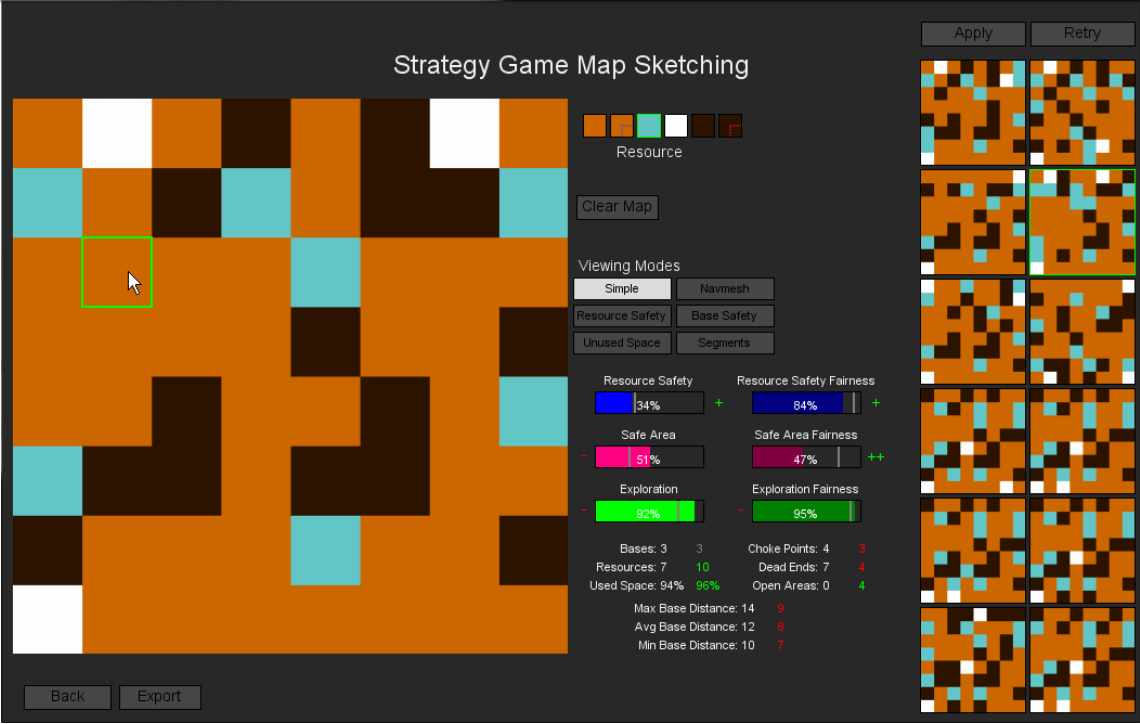
\includegraphics[width=1.0\linewidth]{SentientSketchbook.PNG}
	\caption{Liapis \textit{et al} Sentient Sketchbook during a design session ~\cite{liapis2013sentient}.}
	\label{Sketchbook}
\end{figure} 

\begin{figure}[h]
	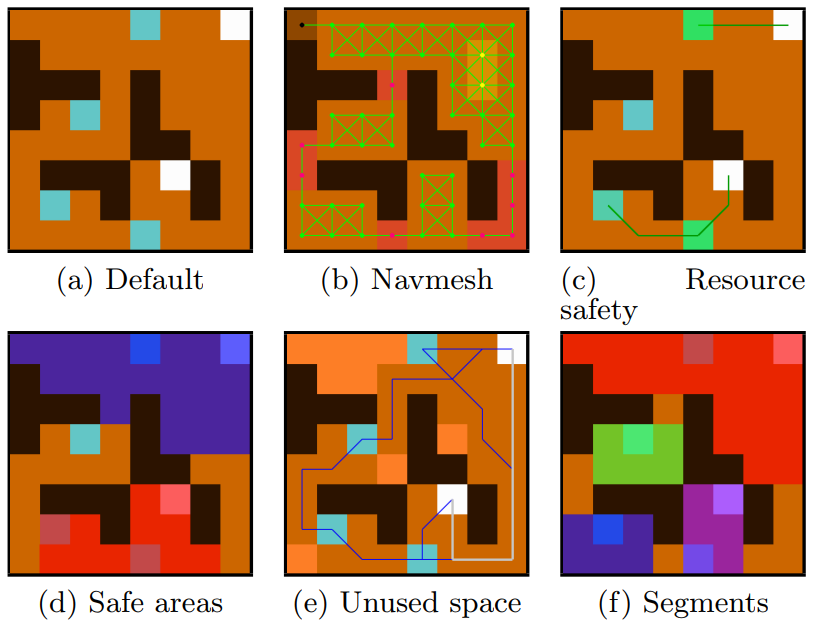
\includegraphics[width=1.0\linewidth]{SentientSketchbook2.PNG}
	\caption{Liapis \textit{et al} Sentient Sketchbook Different viewing modes ~\cite{liapis2013sentient}.}
	\label{Sketchbook2}
\end{figure} 

Baldwin \textit{et al} \cite{baldwin2017mixed} have also implemented a mixed-initiative dungeon designer called the evolutionary dungeon designer or (EDD) for short. EDD is closer to a CAD tool rather than the IE tool Sentient Sketchbook \cite{liapis2013sentient}. While it does allow for large customisation of the levels generated  see Figure~\ref{EDD}  Baldwin \textit{et al} it does take a different approach to Liapis  \textit{et al}\cite{liapis2013sentient} by identifying design patterns within the level design. These design patterns consist of multiple tiles that constitute common patterns found in games. Alvarez \textit{et al}\cite{alvarez2018fostering} builds upon the EDD suggest in \cite{baldwin2017mixed} by adding a IE element to it. It could be argued that the new version of the EDD has an improved interface with lots of its excess drop down menus gone see Figure~\ref{EDD2}. Beyond the ascetic differences, Alvarez \textit{et al}\cite{alvarez2018fostering} dungeon designer integrates key aspects of  the Sentient Sketchpad \cite{liapis2013sentient}. The second edition of the EDD allows the user to design there own levels, it will then offer suggestions based up the map the user created see the top right corner of figure~\ref{EDD2}.  The results from Alvarez \textit{et al}\cite{alvarez2018fostering} experiment focused on whether there tool fostered creativity in the participants using it. Included with the results is a table of requested features made by the participants of the study. One key element highlighted is that the EDD should do a " bit more automated assistance when doing manual designs, which can reduce clicking around the program" \cite[Table 2]{alvarez2018fostering}. Another significant  feature request, was for the dungeon designer to take into account the pattern of the entire dungeon. Using the map of the entire dungeon to generate new rooms.


\begin{figure}[h]
	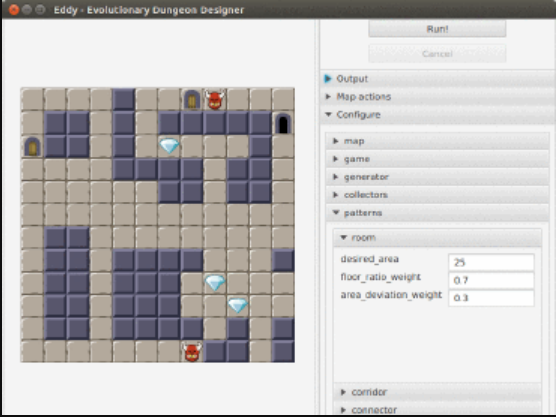
\includegraphics[width=1.0\linewidth]{EDD.PNG}
	\caption{ Baldwin \textit{et al} Evolutionary Dungeon Designer user interface  ~\cite{baldwin2017mixed}.}
	\label{EDD}
\end{figure} 

\begin{figure}[h]
	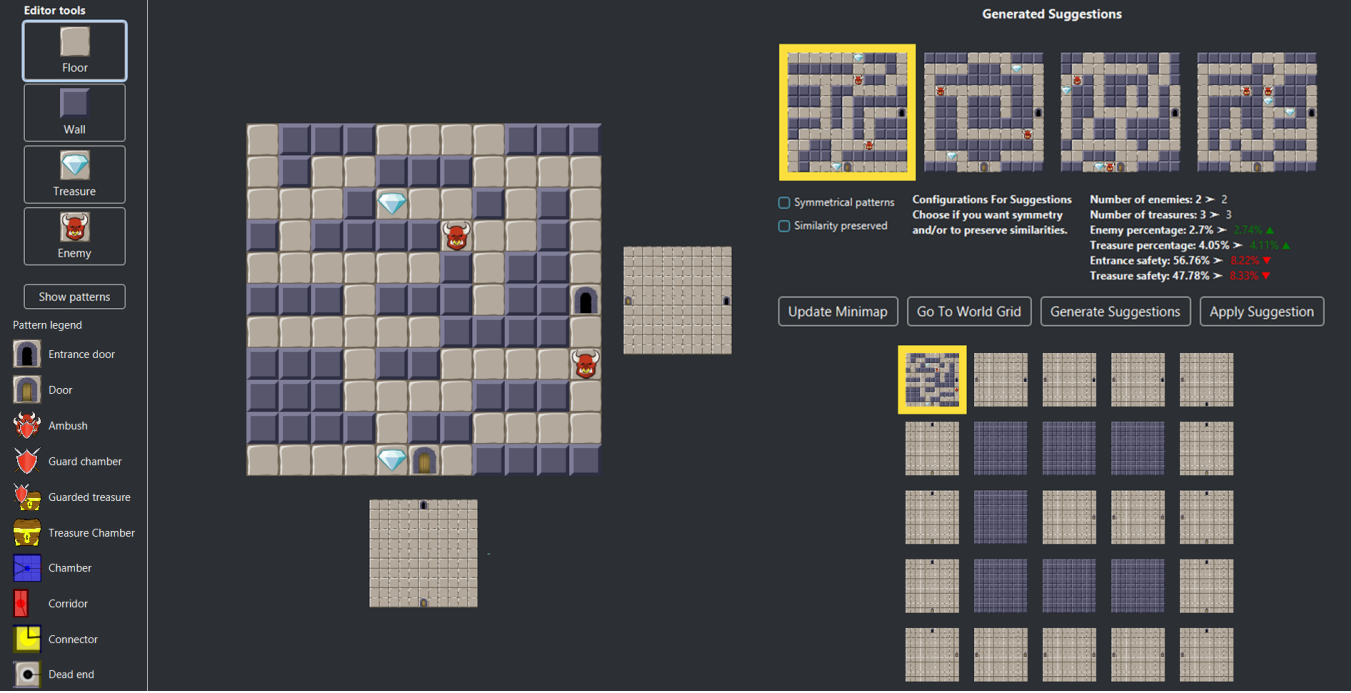
\includegraphics[width=1.0\linewidth]{EDD2.PNG}
	\caption{ Alvarez \textit{et al} Evolutionary Dungeon Designer with modifications user interface  ~\cite{alvarez2018fostering}.}
	\label{EDD2}
\end{figure} 

Horvitz \textit{et al} \cite{horvitz1999principles} propose 12 critical factors to take into consideration when making a mixed-initiative user interface. While Horvitz \textit{et al} \cite{horvitz1999principles}  focuses on an mixed-initiative assistant for Microsoft Outlook (emailing software) it can be argued that some of these factors are relevant for level design .  The first factor that is listed is that a MI tool needs to add significant value through the automation of services. An Examples of a services automated by emailing assistant is the sorting of a users emails into different categories.   Within in the context of \cite{liapis2013sentient}  they satisfy \cite{horvitz1999principles} first critical factor by allowing the computer to automate some of the map design services like checking for broken game constraints. Liapis \textit{et al} \cite{liapis2013sentient} also allow their algorithm take on a creative role all be it based on an original human designed map. Within this project the focus will not be on the creative aspect as the definition of creativity is hard to for a computer to understand \cite{jordanous2010defining}. Alvarez \textit{et al}\cite{alvarez2018fostering} found their MI tool is better at providing controllability than expressivity, when the user imposes their vision, as it is hard for a computer to capture the designers vision. It can be argued that an MI tool could not consistently add value if it cannot capture the designers vision. Gillian \textit{et al}\cite{smith2011tanagra} believe that a human designers strengths lay in creativity and their ability to evaluate good content and the the computer lacks this ability. 

Another factor raised by \cite{horvitz1999principles} is that an MI tool must consider minimizing the costs of poor guesses about the users goals. Even with an extensive history of user goals, novel goals might be implemented during this time the system will benefit from the understanding it cannot predict what the user is trying to accomplish.  Some authors find value in these missed guesses and even seek to find novelty search spaces \cite{liapis2013sentient}. Other authors \cite{liapis2016can,alvarez2018fostering, yannakakis2014mixed} claim these kind of mistakes can foster creativity and alternate suggestions that do not aim to predict the user can be beneficial. On the right hand side of Figure~\ref{Sketchbook} is where the guessing algorithms results are shown. Clicking retry will quickly remove the selected map and create a new one. 

None of the above examples \cite{alvarez2018fostering, liapis2013sentient, baldwin2017mixed} satisfy  Barnes \textit{et al}\cite{barnes2015designing} statement that a mixed-initiative systems UI must provide transparency to the reasoning behind the agents actions. In all cases above\cite{alvarez2018fostering, liapis2013sentient, baldwin2017mixed} , when generating new suggestions the reasoning behind each suggestion was not given to the designer. The designer is presented with the statstics of the current map generated(density, number of resources ETC) but it is not clear from the interface how these statistics are being used. When automating a system transparency is required for a human to trust the automation process \cite{lee2004trust}.

\subsection{Prediction Methods} \label{prediction}
Predictive texting increases the average message length users send to each other \cite{ling2005length} as well as the speed the words are written \cite{dunlop2000predictive}. The same theory may apply to game design. If patterns to a users game design are established, an AI system may be able to assist in design. However, the principle with working with predictive texting is different to that of game design.

The researchers of \cite{chipalkatty2013less} tested alternate methods for predicting human input so as to abstract the low-level movements of the robots the humans were controlling. They built on the idea that humans are good for high-level abstract tasks, but an AI agent was much better at performing low-level repetitive control tasks. They also found that when trying to predict the input the human would do next, trying to identify patterns in a history of inputs was far less successful at predicting the humans intention than just using the last input given by the human. Instead of using current human inputs, \cite{bhatia2016targeted} used the history of the humans social media page to predict the users interests. Perhaps if the authors of \cite{chipalkatty2013less} had looked less at the input history of the human and instead focused on grouping inputs together to create larger actions. Similar, to how modern day phones often predict entire sentences rather than just single words.

Markov Chains is a theory similar to the most successful method found by Bhatia\textit{et al} \cite{bhatia2016targeted}. A Markov chain is a special kind of process that works under the assumption that  the state at time \textit{t+1} depends on the current state or to put it another the state at time \textit{t}. State \textit{t+1}  is not dependent on the history of the states leading up to it\cite{ye2000markov}. While this technique may be useful for predicting anomalies in systems \cite{ju2001hybrid, gwadera2005markov, ye2000markov} where the states are heavily dependent on the latter state happening. It is hard to see how, during a creative process where the next state is dependent on the vision of the designer we can infer state \textit{t+1} just from the state at \textit{t}. 


\section{Methodology}
The research question proposed in this project is: How Will a Mixed-Initiative Level Designer that Predict User Requirements Affect the Size and Speed of the Levels Created?  A discussion of the hypothesis drawn from this question can be view in Section ~\ref{hyp}

\subsection{Creating levels}
The experiment proposed in this paper need at least two dependent variables. Firstly the speed of which a level was created. To measure this, the participants will be restricted in the size of the level they are allowed to create see Table ~\ref{settings} settings 3 and settings 4. Before this first part of the experiment the users will be explained the rules. There will be a minimum number of tiles required before a level is deemed "complete". The designer must place at least one start, one end and one other kind of tile. At least three props will be placed anywhere inside any of the placed rooms. After doing this the level complete button will be available.  The size of the grid presented to the user will be \textit{24 x 24}.

\begin{table}[h]
	\centering
	\caption{Editor Settings}
	\label{settings}
	\def\arraystretch{2}
\resizebox{\columnwidth}{!}{\begin{tabular}{|l|l|l|l|l|}
		\hline
		\textbf{Editor Settings} & \textbf{Predictive Placements Enables}& \textbf{Infinite Level Enabled} \\\hline
		Settings 1  &  X & X \\ \hline
		Settings 2  &     & X \\ \hline
		Settings 3  &   X&  \\ \hline
		Settings 4  &    &  \\ \hline
	\end{tabular}}
\end{table}



\subsection{Hypothesis}\label{hyp}
When creating a level designer the aim is to always increase the ease at which levels could normally be created. For the scope of this paper, we will look not look at how the editor created performs, but how the mixed-initiative tool performs. 

\bibliographystyle{IEEEtran}
\bibliography{references}

% Appendices

\appendices
\section{First appendix}
Appendices are optional. Delete or comment out this part if you do not need them.

% that's all folks
\end{document}
